\documentclass[11pt]{amsart}
\usepackage[a4paper,margin=2.9cm]{geometry}
\usepackage{amssymb,mathtools,booktabs,tikz}
\usepackage[colorlinks=true,linkcolor=blue!60!black,citecolor=green!40!black,urlcolor=blue!60!black]{hyperref}
\usetikzlibrary{calc}

\newtheorem{theorem}{Theorem}[section]
\newtheorem{lemma}[theorem]{Lemma}
\newtheorem{proposition}[theorem]{Proposition}
\newtheorem{corollary}[theorem]{Corollary}
\theoremstyle{definition}
\newtheorem{definition}[theorem]{Definition}
\theoremstyle{remark}
\newtheorem{remark}[theorem]{Remark}

\DeclareMathOperator{\conv}{conv}
\newcommand{\dBM}{d}
\newcommand{\R}{\mathbb R}
\newcommand{\N}{\mathcal N}
\newcommand{\C}{\mathcal C}
\newcommand{\D}{\mathcal D}

\tikzset{rat/.style={x=1cm,y=1.7320508cm}, % (x, y/sqrt3) coordinates drawn to true shape
  pt/.style={circle,fill,inner sep=1.1pt}, opt/.style={circle,draw,fill=white,inner sep=1.1pt}}

\begin{document}

\title{The Banach--Mazur distance between planar convex bodies is at most $11/5$}
\author{Marin Varivoda}
\address{Department of Mathematics, Faculty of Science, University of Zagreb, Bijeni\v{c}ka cesta 30, 10000 Zagreb, Croatia}
\email{marin.varivoda@math.hr}
\date{\today}
\subjclass[2020]{52A10, 52A40, 46B20}
\keywords{Banach--Mazur distance, planar convex bodies, Banach--Mazur compactum, $\varepsilon$-net, computer-assisted proof}

\begin{abstract}
We prove that the Banach--Mazur distance between any two planar convex bodies is at most
$11/5$, improving the bound $(19-\sqrt{73})/4\approx 2.614$ of Brodiuk, Palko and Prymak.
The conjectured maximum is $1+\sqrt5/2\approx2.118$, the distance between a triangle and a
regular pentagon. The proof is computer assisted. We normalise a body by an inscribed affine-regular
hexagon and sort all bodies into finitely many cells, each consisting of the bodies squeezed between two
explicit rational polygons. The bound for every pair of cells is certified by rational witnesses,
which a short independent program verifies in exact rational arithmetic. Along the way we obtain an
explicit $\frac14$-net of the planar Banach--Mazur compactum consisting of $6\,729$ polygons.
\end{abstract}

\maketitle

%==========================================================================
\section{Introduction}

For convex bodies $K,L\subset\R^2$ (compact convex sets with non-empty interior) the
Banach--Mazur distance is
\[
  \dBM(K,L)=\inf\bigl\{\lambda\ge1:\ T(L)\subseteq K\subseteq\lambda T(L)+b,\ T \text{ an invertible affine map},\ b\in\R^2\bigr\}.
\]
It is symmetric and affine invariant, it satisfies $\dBM(K,M)\le\dBM(K,L)\,\dBM(L,M)$, and $\log\dBM$ is a
metric on the set of affine equivalence classes of planar convex bodies, which is compact, the
\emph{(planar) Banach--Mazur compactum}. We are interested in its diameter
\[
  D_2=\sup\{\dBM(K,L):\ K,L\subset\R^2 \text{ convex bodies}\}.
\]
By John's theorem~\cite{John} every planar convex body $K$ satisfies $\dBM(K,B^2)\le2$, hence $D_2\le4$.
Lassak~\cite{Lassak07} proved $D_2\le3$, and Brodiuk, Palko and Prymak~\cite{BPP} proved
$D_2\le\frac{19-\sqrt{73}}4\approx2.614$; this is still listed as the best known planar bound in the recent
work of Brandenberg, Gonz\'alez Merino and Grundbacher~\cite{BGG} on the higher-dimensional problem. On the other
hand, the distance between a triangle $\Delta$ and the regular pentagon $P_5$ is $1+\frac{\sqrt5}2\approx2.118$
(Figure~\ref{fig:sandwich}; see \cite{FMRWY,Lassak92,Kobos}), and Lassak conjectured that this is the diameter,
$D_2=1+\frac{\sqrt5}2$ \cite{Lassak92,Lassak07,Lassak14}. For centrally symmetric bodies the corresponding diameter
is $\frac32$, by a theorem of Stromquist~\cite{Stromquist}, and for a symmetric body $L$ and an arbitrary $K$ one has
$\dBM(K,L)\le2$, with equality only for triangles~\cite{Kobos}. In higher dimensions the order of the diameter of the
compactum of not necessarily symmetric bodies is known up to logarithmic factors~\cite{Rudelson00,BK}.

\begin{theorem}\label{thm:main}
For all planar convex bodies $K$ and $L$,\quad $\dBM(K,L)\le\dfrac{11}{5}$.
\end{theorem}

In particular every planar convex body $K$ contains a triangle $T$ with $K\subseteq c+\frac{11}5(T-c)$ for some $c$; to
our knowledge the best previous constant for this was $\frac94$, due to Fleischer, Mehlhorn, Rote, Welzl and
Yap~\cite{FMRWY}.

\begin{figure}[t]
\centering
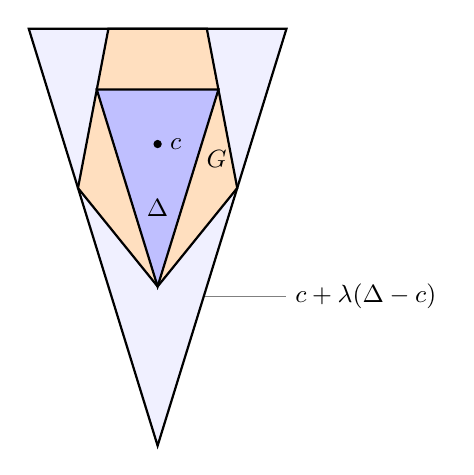
\begin{tikzpicture}[scale=1.25]
  \draw[thick,fill=blue!6] (0,-1.618) -- (1.309,2.618) -- (-1.309,2.618) -- cycle;
  \draw[thick,fill=orange!25] (0,0) -- (0.809,1) -- (0.5,2.618) -- (-0.5,2.618) -- (-0.809,1) -- cycle;
  \draw[thick,fill=blue!25] (0,0) -- (0.618,2) -- (-0.618,2) -- cycle;
  \fill (0,1.447) circle (1.2pt) node[right=1pt,font=\small] {$c$};
  \node[font=\small] at (0,0.8) {$\Delta$};
  \node[font=\small] at (0.6,1.3) {$G$};
  \draw[gray] (0.48,-0.1) -- (1.3,-0.1) node[right,font=\small,black] {$c+\lambda(\Delta-c)$};
\end{tikzpicture}
\caption{An optimal sandwich for a triangle and a regular pentagon: $\Delta\subseteq G\subseteq c+\lambda(\Delta-c)$ with
$G$ an affine-regular pentagon and $\lambda=1+\frac{\sqrt5}2$.}
\label{fig:sandwich}
\end{figure}

\subsection*{Method}
The proof has a short geometric part and a large but elementary computational part.
By a theorem of Besicovitch~\cite{Besicovitch} every planar convex body $K$ has an inscribed affine-regular
hexagon; after an affine map it is a fixed regular hexagon $H$, and then $K$ lies in the hexagram formed by $H$
and the six equilateral triangles erected on its sides. In each of these triangles we use two slopes as
coordinates; in them, the relevant geometry becomes a matter of comparing coordinates
(Section~\ref{sec:frame}).
Six points over each side define a finite family of polygons $\N$ with $6\,729$ members up to symmetry, and every
convex body is within distance $\frac54$ of a member of $\N$ (Theorem~\ref{thm:net}). This
already gives $D_2\le\frac{25}{16}\max_{P,Q\in\N}\dBM(P,Q)$.

For the bound $\frac{11}5$ we use the net in a sharper form. Recording which of the six points over each side lie in
$K$ places $K$ in a \emph{cell}, all of whose bodies $K$ satisfy $P\subseteq K\subseteq O$ for two explicit
rational polygons $P$ and $O$ (Section~\ref{sec:cells}). A single linear map that fits the polygons of two cells
into each other bounds $\dBM(K,L)$ for all bodies $K,L$ of these cells (Proposition~\ref{prop:cellbound}). Bounds through
$60$ fixed ``hub'' polygons handle all but $1\,339$ of the $22\,643\,085$ pairs of cells, and each remaining pair is handled
by splitting its cells on new points until every piece has such a bound; in all, $433\,821$ witnesses are used. The witnesses are found in floating point and then
rounded to rationals. The resulting certificate is checked by an independent program that recomputes all cells and
verifies every witness in exact rational arithmetic (Section~\ref{sec:proof}). The code and the
certificate are available at \url{https://github.com/marin-varivoda/planar-bm-diameter}.

\subsection*{Related work}
Zong~\cite{Zong10} proposed a computer-assisted programme for Hadwiger's covering conjecture based on finite nets of
the Banach--Mazur compactum, and proved that such nets exist for convex bodies in every dimension; see also
\cite{GMWZ}. The asymptotic size of optimal nets is governed by the metric entropy of the compactum, estimated by
Bronshtein~\cite{Bronshtein} (and in high dimensions by Pisier~\cite{Pisier}); see also the discussion in
Kobos and Swanepoel~\cite{KS}. Chen, Lyu, Gao and Wu~\cite{CLGW} constructed an explicit $\frac14$-net of the
\emph{centrally symmetric} planar convex bodies from lattice polygons, and described an algorithm for general planar
bodies. To our knowledge, the net of Theorem~\ref{thm:net} is the first explicit $\varepsilon$-net of the compactum of
all, not necessarily symmetric, planar convex bodies; it is built on the inscribed hexagon rather than on lattice polygons.
Numerical computations have also guided work on other Banach--Mazur problems, for instance on the distance between
the cube and the cross-polytope~\cite{Xue}, whose values in dimensions $3$ and $4$ were then established in~\cite{KV}.

%==========================================================================
\section{The hexagon frame}\label{sec:frame}

\subsection{Coordinates}
Since $\dBM$ is affine invariant we may use the coordinates $(x,y/\sqrt3)$, in which all relevant points are
rational. All figures are drawn to true shape. Let
\[
  H=\conv\{(\pm1,0),(\pm2,-1),(\pm1,-2)\},\qquad I=(0,-1),
\]
the regular hexagon with centre $I$, and let $\rho$ be the rotation by $60^\circ$ about $I$; in these coordinates
$\rho(I+(x,y))=I+\bigl(\frac{x-3y}2,\frac{x+y}2\bigr)$. The sides of $H$ are $s_k=\rho^k(s_0)$, $k\in\mathbb Z/6$, where
$s_0=[B,C]$ with $B=(-1,0)$ and $C=(1,0)$. Write $B_k=\rho^k(B)$ and $C_k=\rho^k(C)$; then $B_k=C_{k+1}$. Over $s_0$ we
erect the equilateral triangle $\Delta_0=\conv\{B,C,A\}$, $A=(0,1)$, and put $\Delta_k=\rho^k(\Delta_0)$.

\begin{lemma}[Besicovitch~\cite{Besicovitch}]\label{lem:besicovitch}
Every planar convex body $K$ has an inscribed affine-regular hexagon, i.e.\ an affine image of $H$ whose six vertices lie
on $\partial K$.
\end{lemma}

We call $K$ \emph{normalised} if all vertices of $H$ lie on $\partial K$ (so $H\subseteq K$). By
Lemma~\ref{lem:besicovitch} every convex body is affinely equivalent to a normalised one.

\begin{lemma}\label{lem:hexagram}
If $K$ is normalised, then $K\subseteq H\cup\Delta_0\cup\dots\cup\Delta_5$.
\end{lemma}

\begin{proof}
Let $p\in K\setminus H$. The sides of $H$ whose lines separate $p$ from $H$ form a non-empty set of consecutive sides. If
it contained two consecutive sides, say $s_0$ and $s_1$ meeting at $B$, then $p-B=-\alpha(C-B)-\beta(B_1-B)$ with
$\alpha,\beta>0$, so $B$ would be a positive convex combination of $p$, $C$ and $B_1$, hence an interior point of $K$. So
the line of only one side separates $p$ from $H$, say that of $s_0$, and then $p\in\Delta_0$, because the lines of $s_1$
and $s_5$ meet at $A$.
\end{proof}

\subsection{Slopes}
For a point $q=(x,y)$ with $y>0$ and $|x|<1$ put
\[
  a(q)=\frac{y}{1+x},\qquad b(q)=\frac{y}{1-x}.
\]
In true shape, $\sqrt3\,a(q)$ and $\sqrt3\,b(q)$ are the tangents of the angles $\angle qBC$ and $\angle qCB$. The
map $q\mapsto(a(q),b(q))$ is a bijection from $\Delta_0\setminus s_0$ onto the \emph{slope square} $(0,1]^2$, with inverse
\[
  q(a,b)=\Bigl(\frac{b-a}{a+b},\ \frac{2ab}{a+b}\Bigr),
\]
and we put $q_k=\rho^k\circ q$, the point with slopes $(a,b)$ over the side $s_k$. We order slope points componentwise:
$z\le z'$ ($z'$ \emph{dominates} $z$) if $a\le a'$ and $b\le b'$. Since the triangle $\conv\{B,C,q\}$ is cut out by
$y\ge0$ and the lines $Bq$ and $Cq$,
\begin{equation}\label{eq:dominance}
  q(z)\in\conv\{B,C,q(z')\}\iff z\le z' .
\end{equation}
For a normalised body $K$ let $Z_k(K)=\{z\in(0,1]^2: q_k(z)\in K\}$ be the set of slopes of the points of $K$ over $s_k$.
By Lemma~\ref{lem:hexagram},
\begin{equation}\label{eq:profile}
  K=H\cup q_0(Z_0(K))\cup\dots\cup q_5(Z_5(K)),
\end{equation}
and since $B_k,C_k\in K$, \eqref{eq:dominance} and convexity show that each $Z_k(K)$ is a \emph{down-set}: if $z\in Z_k(K)$
and $z'\le z$, then $z'\in Z_k(K)$. The last ingredient is a condition at the vertices of $H$, which lie on $\partial K$.
Let
\[
  m(t)=\frac{1-t}{1+3t}\qquad(0\le t\le1),
\]
a decreasing bijection of $[0,1]$ with $m(m(t))=t$.

\begin{lemma}[vertex condition]\label{lem:vertex}
Let $K$ be normalised, $z\in Z_k(K)$ and $z'\in Z_{k+1}(K)$. Then $a(z)\le m(b(z'))$, equivalently
$a(z)+b(z')+3a(z)b(z')\le1$.
\end{lemma}

\begin{proof}
Work in true shape at the vertex $V=B_k=C_{k+1}\in\partial K$. The directions from $V$ to $q_k(z)$, $C_k$, $B_{k+1}$
and $q_{k+1}(z')$ occur in this angular order, with consecutive angles $\alpha=\arctan(\sqrt3a)$, $120^\circ$ and
$\beta=\arctan(\sqrt3b')$, where $a=a(z)$, $b'=b(z')$ and $\alpha,\beta\le60^\circ$. All four points lie in $K$, and a
supporting line of $K$ at $V$ puts the four directions into a closed half-plane. Hence $\alpha+\beta\le60^\circ$, and
$\sin(60^\circ-\alpha-\beta)=\tfrac{\sqrt3}2\cos\alpha\cos\beta\,(1-a-b'-3ab')$.
\end{proof}

%==========================================================================
\section{A $\frac14$-net}\label{sec:net}

Over each side we use the six slope points
\begin{center}
\begin{tabular}{lcccccc}
\toprule
point & $Y$ & $S$ & $T$ & $U$ & $V$ & $X$\\
\midrule
slopes $(a,b)$ & $(\frac17,\frac17)$ & $(\frac13,\frac17)$ & $(\frac17,\frac13)$ & $(\frac12,\frac13)$ & $(\frac13,\frac12)$ & $(\frac35,\frac35)$\\[2pt]
position over $s_0$ & $(0,\frac17)$ & $(-\frac25,\frac15)$ & $(\frac25,\frac15)$ & $(-\frac15,\frac25)$ & $(\frac15,\frac25)$ & $(0,\frac35)$\\
\bottomrule
\end{tabular}
\end{center}
shown in Figure~\ref{fig:frame}; for instance $X$ is the image of $A$ under the homothety $F(q)=I+\frac45(q-I)$. In the
dominance order $Y<S,T<U,V<X$, with $S,T$ and $U,V$ incomparable. For a normalised $K$ the net points in $Z_k(K)$ form a
down-set of the net. There are nine down-sets, the \emph{patches}, which we name by their maximal elements:
\[
  0,\ Y,\ S,\ T,\ ST,\ U,\ V,\ UV,\ X .
\]
For a patch $p$ let $l(p)$ and $r(p)$ be the largest $a$- and $b$-slope of its points ($0$ for the empty
patch~$0$). A \emph{configuration} is a sequence $\mathbf p=(p_0,\dots,p_5)$ of patches; it is \emph{admissible} if
$l(p_k)\le m(r(p_{k+1}))$ for all $k\in\mathbb Z/6$, and then $P(\mathbf p)$ is the convex hull of $H$ and of the points of
$p_k$ over $s_k$, $k=0,\dots,5$. By Lemma~\ref{lem:vertex}, the configuration $\mathbf p(K)$ of the net points in a
normalised body $K$ is admissible.

\begin{figure}[t]
\centering
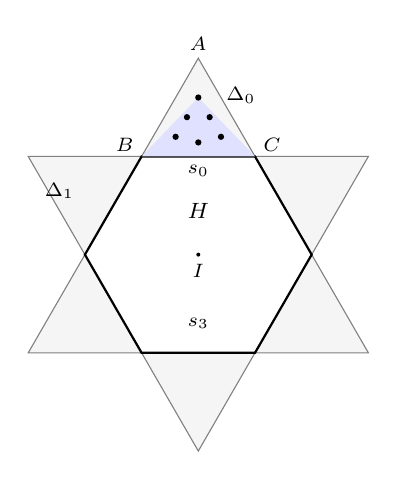
\begin{tikzpicture}[rat,scale=0.72]
  \fill[gray!8] (0,1)--(-1,0)--(-3,0)--(-2,-1)--(-3,-2)--(-1,-2)--(0,-3)--(1,-2)--(3,-2)--(2,-1)--(3,0)--(1,0)--cycle;
  \draw[gray] (0,1)--(-1,0)--(-3,0)--(-2,-1)--(-3,-2)--(-1,-2)--(0,-3)--(1,-2)--(3,-2)--(2,-1)--(3,0)--(1,0)--cycle;
  \draw[thick,fill=white] (1,0)--(-1,0)--(-2,-1)--(-1,-2)--(1,-2)--(2,-1)--cycle;
  \fill[blue!12] (-1,0)--(0,0.6)--(1,0)--cycle;
  \foreach \p in {(0,0.142857),(-0.4,0.2),(0.4,0.2),(-0.2,0.4),(0.2,0.4),(0,0.6)} \node[pt,inner sep=0.8pt] at \p {};
  \node[font=\footnotesize] at (0,-0.55) {$H$};
  \fill (0,-1) circle (1pt) node[below,font=\scriptsize] {$I$};
  \node[font=\scriptsize] at (0,1.15) {$A$};
  \node[font=\scriptsize] at (-1.3,0.12) {$B$};
  \node[font=\scriptsize] at (1.3,0.12) {$C$};
  \node[font=\scriptsize] at (-2.45,-0.35) {$\Delta_1$};
  \node[font=\scriptsize] at (0.75,0.62) {$\Delta_0$};
  \node[font=\scriptsize] at (0,-1.7) {$s_3$};
  \node[font=\scriptsize] at (0,-0.15) {$s_0$};
\end{tikzpicture}\hfill
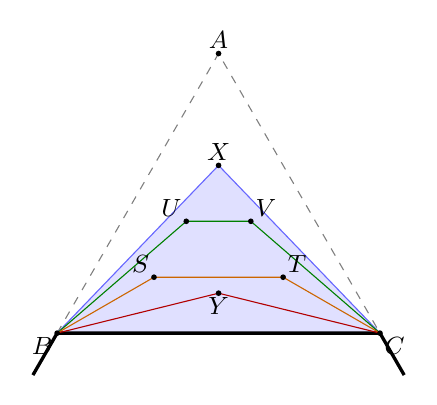
\begin{tikzpicture}[rat,scale=2.05]
  \draw[gray,dashed] (-1,0)--(0,1)--(1,0);
  \fill[blue!12] (-1,0)--(0,0.6)--(1,0)--cycle;
  \draw[very thick] (-1.15,-0.15)--(-1,0)--(1,0)--(1.15,-0.15);
  \draw[blue!60] (-1,0)--(0,0.6)--(1,0);
  \draw[green!50!black] (-1,0)--(-0.2,0.4)--(0.2,0.4)--(1,0);
  \draw[orange!80!black] (-1,0)--(-0.4,0.2)--(0.4,0.2)--(1,0);
  \draw[red!70!black] (-1,0)--(0,1/7)--(1,0);
  \foreach \p/\n/\pos in {(-1,0)/B/below left,(1,0)/C/below right,(0,1)/A/above,(0,0.6)/X/above,
     (-0.2,0.4)/U/above left,(0.2,0.4)/V/above right,(-0.4,0.2)/S/above left,(0.4,0.2)/T/above right,(0,0.142857)/Y/below}
    {\fill \p circle (0.5pt); \node[\pos,font=\small,inner sep=1.5pt] at \p {$\n$};}
\end{tikzpicture}\hfill
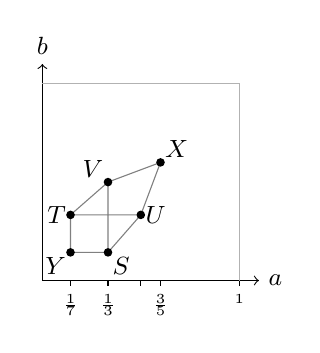
\begin{tikzpicture}[scale=2.5]
  \draw[->] (0,0)--(1.1,0) node[right,font=\small] {$a$};
  \draw[->] (0,0)--(0,1.1) node[above,font=\small] {$b$};
  \draw[gray!60] (1,0)--(1,1)--(0,1);
  \foreach \v/\l in {0.142857/\frac17,0.333333/\frac13,0.6/\frac35,1}
     {\draw (\v,0)--(\v,-0.03); \node[below,font=\tiny] at (\v,-0.02) {$\l$};}
  \draw (0.5,0)--(0.5,-0.03);
  \draw[gray] (1/7,1/7)--(1/3,1/7)--(1/2,1/3)--(3/5,3/5) (1/7,1/7)--(1/7,1/3)--(1/3,1/2)--(3/5,3/5) (1/3,1/7)--(1/3,1/2) (1/7,1/3)--(1/2,1/3);
  \foreach \p/\n/\pos in {(0.142857,0.142857)/Y/below left,(0.333333,0.142857)/S/below right,(0.142857,0.333333)/T/left,(0.5,0.333333)/U/right,(0.333333,0.5)/V/above left,(0.6,0.6)/X/above right}
    {\node[pt] at \p {}; \node[\pos,font=\small,inner sep=1.5pt] at \p {$\n$};}
\end{tikzpicture}
\caption{Left: the hexagon $H$ and the hexagram $H\cup\Delta_0\cup\dots\cup\Delta_5$ containing every normalised
body (Lemma~\ref{lem:hexagram}); the net points over $s_0$. Middle: the triangle $\Delta_0$ with the net points and some
patches; shaded is the largest patch $X$. Right: the net points in slope coordinates, with the dominance order.}
\label{fig:frame}
\end{figure}

\begin{proposition}\label{prop:count}
There are $77\,625$ admissible configurations. The dihedral group $D_6$ of symmetries of $H$ acts on them
(a rotation shifts the indices, a reflection reverses them and exchanges $S\leftrightarrow T$ and
$U\leftrightarrow V$), with $6\,729$ orbits.
\end{proposition}

\begin{proof}
Enumeration (\texttt{proof.py}). As a check, by Burnside's lemma: the identity, the rotations by $\pm60^\circ$,
$\pm120^\circ$, $180^\circ$, the three reflections in lines through midpoints of opposite sides and the three in lines
through opposite vertices fix $77\,625$, $5$, $45$, $275$, $711$ and $205$ configurations each, and
$\frac1{12}(77\,625+2\cdot5+2\cdot45+275+3\cdot711+3\cdot205)=6\,729$.
\end{proof}

\begin{theorem}\label{thm:net}
If $K$ is normalised, then
$P(\mathbf p(K))\subseteq K\subseteq I+\tfrac54\bigl(P(\mathbf p(K))-I\bigr)$.
Consequently the polygons $P(\mathbf p)$, $\mathbf p$ admissible, form a $\frac14$-net of the planar Banach--Mazur
compactum: every planar convex body is within distance $\frac54$ of one of them, and there are at most $6\,729$ of
them up to affine equivalence.
\end{theorem}

\begin{proof}
$P=P(\mathbf p(K))\subseteq K$ by convexity. For the second inclusion we show $F(K)\subseteq P$ for
$F(q)=I+\frac45(q-I)$. As $F(H)\subseteq H$, by \eqref{eq:profile} and symmetry it suffices to show $F(q)\in P$ for
$q\in K\cap\Delta_0\setminus s_0$. All net points dominated by the slopes of $q$ lie in $K$, hence in $P$, so it suffices that
\[
  F(q)\in\conv\bigl(H\cup\{\text{net points over $s_0$ dominated by the slopes of }q\}\bigr)\qquad\text{for all }q\in\Delta_0\setminus s_0 .
\]
Cut the slope square along $a,b\in\{\frac17,\frac13,\frac12,\frac35\}$ into $25$ rectangles $[a_0,a_1]\times[b_0,b_1]$. For
$q$ in such a rectangle the right-hand side contains the polygon $P_{a_0b_0}$ spanned by $H$ and the net points
$z\le(a_0,b_0)$. The points with slopes in the rectangle form the quadrilateral bounded by the lines through $B$ with
$a\in\{a_0,a_1\}$ and the lines through $C$ with $b\in\{b_0,b_1\}$, with vertices $q(a,b)$, $a\in\{a_0,a_1\}$,
$b\in\{b_0,b_1\}$ (a vertex with $a=0$ or $b=0$ is $C$ or $B$, or both). As $F$ is affine and $F(B),F(C)\in H$, it suffices
to check $F(q(a,b))\in P_{a_0b_0}$ for the vertices with $a,b>0$. These are finitely many exact point-in-polygon
tests, which all succeed (\texttt{proof.py}). Several are tight, e.g.\ $F(A)=X$.
\end{proof}

\begin{remark}
By the multiplicative triangle inequality, Theorem~\ref{thm:net} gives $D_2\le\frac{25}{16}m^*$, where $m^*$ is the largest
distance between two members of the net. Numerically $m^*\approx1.6145$, attained between $P(0,X,0,X,0,X)$, the member closest
to a triangle, and $P(Y,Y,T,V,U,S)$; a certified bound of this kind would give $D_2<2.53$. We do not use this route: the
proof of Theorem~\ref{thm:main} uses the net points, but not the factor $\frac54$.
\end{remark}

%==========================================================================
\section{Cells}\label{sec:cells}

A cell records some slope points that lie in a body and some that do not. It is then squeezed between two polygons.

\begin{definition}\label{def:cell}
A \emph{cell} $\C$ consists of finite sets $I_k,E_k\subset(0,1)^2$ of slope points, $k\in\mathbb Z/6$ (``inside'' and
``outside''). A normalised body $K$ \emph{belongs} to $\C$ if $I_k\subseteq Z_k(K)$ and $E_k\cap Z_k(K)=\emptyset$ for all $k$.
The \emph{inner polygon} $P(\C)$ is the convex hull of $H$ and of the points $q_k(z)$, $z\in I_k$. Let $l_k$ and $r_k$ be the
largest $a$- and $b$-slope in $I_k$ ($0$ if $I_k=\emptyset$), and let the \emph{staircase} $S_k$ be the set of
$(a,b)\in[0,m(r_{k+1})]\times[0,m(l_{k-1})]$ such that $a\le a_e$ or $b\le b_e$ for every $(a_e,b_e)\in E_k$. The
\emph{outer polygon} $O(\C)$ is the convex hull of $H$ and of the points $q_k(c)$ for the corners $c$ of the staircases
$S_k$ (Figure~\ref{fig:staircase}).
\end{definition}

The \emph{corners} of $S_k$ are its maximal points; every point of $S_k$ is dominated by a corner. Their coordinates
are among $m(r_{k+1})$ and the $a_e$, resp.\ $m(l_{k-1})$ and the $b_e$, so there are finitely many.

\begin{lemma}\label{lem:cell}
If $K$ belongs to the cell $\C$, then $P(\C)\subseteq K\subseteq O(\C)$.
\end{lemma}

\begin{proof}
The first inclusion holds by convexity. For the second, by \eqref{eq:profile} it suffices to show that every
$w=(a,b)\in Z_k(K)$ lies in $S_k$: then $w$ is dominated by a corner $c$, and $q_k(w)\in\conv\{B_k,C_k,q_k(c)\}\subseteq O(\C)$
by \eqref{eq:dominance}. As $Z_k(K)$ is a down-set that does not contain any $e\in E_k$, $w$ does not dominate $e$, so
$a<a_e$ or $b<b_e$. And by Lemma~\ref{lem:vertex}, applied to $w$ and a point of $I_{k+1}$ with $b$-slope $r_{k+1}$, and to a point of
$I_{k-1}$ with $a$-slope $l_{k-1}$ and $w$, we have $a\le m(r_{k+1})$ and $b\le m(l_{k-1})$.
\end{proof}

\begin{figure}[t]
\centering
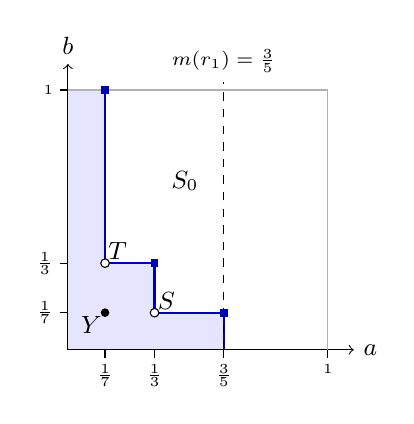
\begin{tikzpicture}[scale=3.3]
  \fill[blue!10] (0,0)--(0,1)--(1/7,1)--(1/7,1/3)--(1/3,1/3)--(1/3,1/7)--(3/5,1/7)--(3/5,0)--cycle;
  \draw[blue!70!black,thick] (0,1)--(1/7,1)--(1/7,1/3)--(1/3,1/3)--(1/3,1/7)--(3/5,1/7)--(3/5,0);
  \draw[->] (0,0)--(1.1,0) node[right,font=\small] {$a$};
  \draw[->] (0,0)--(0,1.1) node[above,font=\small] {$b$};
  \draw[gray!60] (1,0)--(1,1)--(0,1);
  \draw[dashed] (3/5,0)--(3/5,1.03) node[above,font=\scriptsize] {$m(r_1)=\frac35$};
  \foreach \v/\l in {0.142857/\frac17,0.333333/\frac13,0.6/\frac35,1}
     {\draw (\v,0)--(\v,-0.03); \node[below,font=\tiny] at (\v,-0.02) {$\l$};}
  \foreach \v/\l in {0.142857/\frac17,0.333333/\frac13,1}
     {\draw (0,\v)--(-0.03,\v); \node[left,font=\tiny] at (-0.02,\v) {$\l$};}
  \node[pt] at (1/7,1/7) {}; \node[below left,font=\small,inner sep=1pt] at (1/7,1/7) {$Y$};
  \node[opt] at (1/3,1/7) {}; \node[above right,font=\small,inner sep=1pt] at (1/3,1/7) {$S$};
  \node[opt] at (1/7,1/3) {}; \node[above right,font=\small,inner sep=1pt] at (1/7,1/3) {$T$};
  \foreach \p in {(0.142857,1),(0.333333,0.333333),(0.6,0.142857)} \node[blue!70!black,rectangle,fill,inner sep=1.4pt] at \p {};
  \node[font=\small] at (0.45,0.65) {$S_0$};
\end{tikzpicture}\qquad
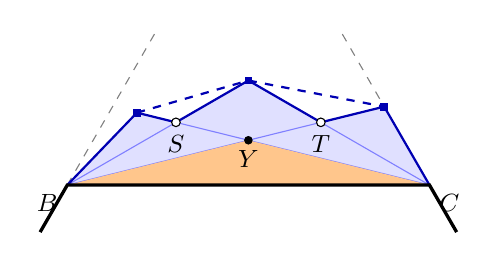
\begin{tikzpicture}[rat,scale=2.3]
  \draw[gray,dashed] (-1,0)--(-0.5,0.5) (1,0)--(0.5,0.5);
  \fill[blue!12] (-1,0)--(-8/13,3/13)--(-0.4,0.2)--(0,1/3)--(0.4,0.2)--(3/4,1/4)--(1,0)--cycle;
  \draw[blue!50,thin] (-1,0)--(0,1/3)--(1,0) (-1,0)--(3/4,1/4) (-8/13,3/13)--(1,0);
  \draw[blue!70!black,thick] (-1,0)--(-8/13,3/13)--(-0.4,0.2)--(0,1/3)--(0.4,0.2)--(3/4,1/4)--(1,0);
  \draw[blue!70!black,thick,dashed] (-8/13,3/13)--(0,1/3)--(3/4,1/4);
  \fill[orange!45] (-1,0)--(0,1/7)--(1,0)--cycle;
  \draw[very thick] (-1.15,-0.15)--(-1,0)--(1,0)--(1.15,-0.15);
  \node[pt] at (0,1/7) {}; \node[below,font=\small] at (0,1/7) {$Y$};
  \node[opt] at (-0.4,0.2) {}; \node[opt] at (0.4,0.2) {};
  \node[below,font=\small] at (-0.4,0.19) {$S$}; \node[below,font=\small] at (0.4,0.19) {$T$};
  \foreach \p in {(-0.615385,0.230769),(0,0.333333),(0.75,0.25)} \node[blue!70!black,rectangle,fill,inner sep=1.4pt] at \p {};
  \node[below left,font=\small] at (-1,0) {$B$}; \node[below right,font=\small] at (1,0) {$C$};
\end{tikzpicture}
\caption{The staircase $S_0$ for $I_0=\{Y\}$, $E_0=\{S,T\}$, $r_1=\frac17$ and $l_5=0$ (left), and its image over the
side $s_0$ (right): the part over $s_0$ of every body of the cell lies in the union (light) of the triangles
$\conv\{B,C,q(c)\}$ over the three corners $c$ (squares), and it contains the triangle $\conv\{B,C,q(Y)\}$ (dark). The outer
polygon uses the convex hull (dashed).}
\label{fig:staircase}
\end{figure}

Every admissible configuration $\mathbf p$ defines a \emph{root cell} $\C(\mathbf p)$: $I_k$ consists of the net points of $p_k$ and
$E_k$ of the other net points. Its inner polygon is $P(\mathbf p)$. Figure~\ref{fig:cells} shows two root cells.

\begin{lemma}\label{lem:roots}
Every planar convex body is affinely equivalent to a body that belongs to one of the $6\,729$ root cells of the
representatives of Proposition~\ref{prop:count}.
\end{lemma}

\begin{proof}
We may assume that $K$ is normalised; it belongs to $\C(\mathbf p(K))$, and $\mathbf p(K)$ is admissible. A symmetry
$g\in D_6$ of $H$ fixes $I$, maps $\Delta_k$ to $\Delta_{g(k)}$ and preserves the slopes, except that reflections exchange
$a$ and $b$. So $g(K)$ is normalised and belongs to $\C(g\mathbf p(K))$, with $D_6$ acting on configurations as in
Proposition~\ref{prop:count}. Choose $g$ with $g\mathbf p(K)$ the representative of its orbit.
\end{proof}

\begin{figure}[t]
\centering
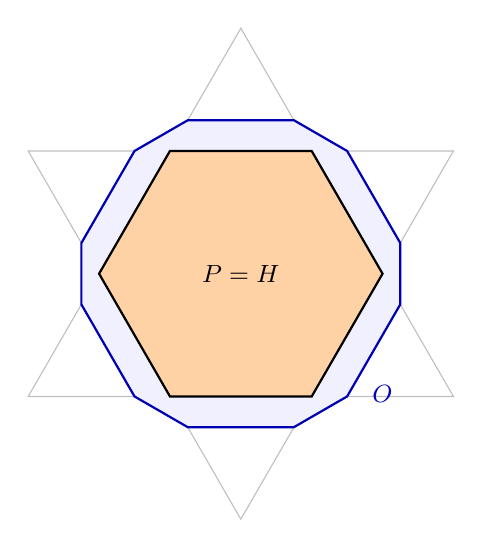
\begin{tikzpicture}[rat,scale=0.9]
  \draw[gray!50] (0,1)--(-1,0)--(-3,0)--(-2,-1)--(-3,-2)--(-1,-2)--(0,-3)--(1,-2)--(3,-2)--(2,-1)--(3,0)--(1,0)--cycle;
  \draw[thick,blue!70!black,fill=blue!6] (-2.25,-1.25)--(-1.5,-2)--(-0.75,-2.25)--(0.75,-2.25)--(1.5,-2)--(2.25,-1.25)--(2.25,-0.75)--(1.5,0)--(0.75,0.25)--(-0.75,0.25)--(-1.5,0)--(-2.25,-0.75)--cycle;
  \draw[thick,fill=orange!35] (1,0)--(-1,0)--(-2,-1)--(-1,-2)--(1,-2)--(2,-1)--cycle;
  \node[font=\small] at (0,-1) {$P=H$};
  \node[font=\small,blue!70!black] at (2.0,-1.98) {$O$};
\end{tikzpicture}\qquad
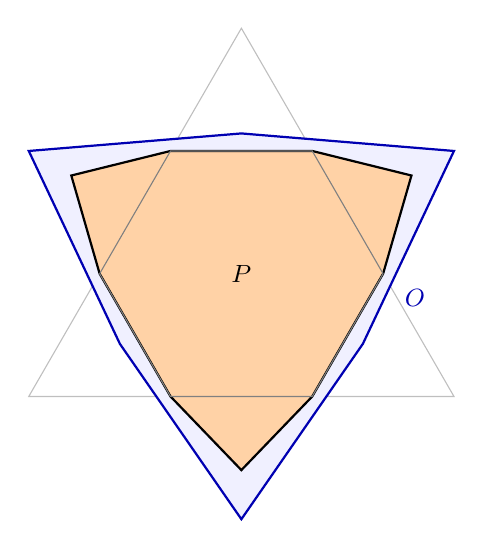
\begin{tikzpicture}[rat,scale=0.9]
  \draw[gray!50] (0,1)--(-1,0)--(-3,0)--(-2,-1)--(-3,-2)--(-1,-2)--(0,-3)--(1,-2)--(3,-2)--(2,-1)--(3,0)--(1,0)--cycle;
  \draw[thick,blue!70!black,fill=blue!6] (-3,0)--(-12/7,-11/7)--(0,-3)--(12/7,-11/7)--(3,0)--(0,1/7)--cycle;
  \draw[thick,fill=orange!35] (-2.4,-0.2)--(-2,-1)--(-1,-2)--(0,-2.6)--(1,-2)--(2,-1)--(2.4,-0.2)--(1,0)--(-1,0)--cycle;
  \draw[gray] (1,0)--(-1,0)--(-2,-1)--(-1,-2)--(1,-2)--(2,-1)--cycle;
  \node[font=\small] at (0,-1) {$P$};
  \node[font=\small,blue!70!black] at (2.45,-1.2) {$O$};
\end{tikzpicture}
\caption{The root cells of the configurations $(0,0,0,0,0,0)$ (left) and $(0,X,0,X,0,X)$ (right): every normalised body $K$
whose net points are exactly those of the configuration satisfies $P\subseteq K\subseteq O$. The right cell contains the triangle
$\conv\{(-3,0),(3,0),(0,-3)\}$.}
\label{fig:cells}
\end{figure}

A cell can be refined. \emph{Splitting} the cell $\C$ on a slope point $z$ over the side $s_k$ gives the two cells $\C^+$ and
$\C^-$ obtained by adding $z$ to $I_k$, resp.\ to $E_k$. Every body of $\C$ belongs to $\C^+$ or to $\C^-$.

%==========================================================================
\section{The proof}\label{sec:proof}

\begin{proposition}\label{prop:cellbound}
Let $\C$, $\D$ be cells, $M$ a linear map, $t,s\in\R^2$ and $\lambda>0$ with
\[
  M\,O(\D)+t\subseteq P(\C)\qquad\text{and}\qquad O(\C)\subseteq\lambda M\,P(\D)+s .
\]
Then $\dBM(K,L)\le\lambda$ for every body $K$ of $\C$ and every body $L$ of $\D$.
\end{proposition}

\begin{proof}
$M$ is invertible, as $\lambda MP(\D)$ contains a translate of $O(\C)$, which has interior points. By Lemma~\ref{lem:cell},
$M L+t\subseteq M\,O(\D)+t\subseteq P(\C)\subseteq K\subseteq O(\C)\subseteq\lambda M\,P(\D)+s\subseteq\lambda ML+s$,
and $\lambda ML+s=\lambda(ML+t)+(s-\lambda t)$.
\end{proof}

We call $(M,t,s,\lambda)$ a \emph{witness} of value $\lambda$ for the pair $(\C,\D)$. The same holds with a fixed convex
polygon $Q$ in place of $\D$, with $P(\D)=O(\D)=Q$ and $L=Q$. All polygons involved have rational vertices, so a
rational witness can be verified exactly: it suffices to check that each vertex of $M\,O(\D)+t$ lies in $P(\C)$ and that each
vertex of $O(\C)$ lies in $\lambda MP(\D)+s$.

Witnesses for all of the $22\,643\,085$ pairs of root cells would be costly, and some pairs need more than one
witness. We use two devices. The first is the triangle inequality: if $\dBM(K,Q)\le e$ and $\dBM(L,Q)\le e'$, then
$\dBM(K,L)\le ee'$. The second is splitting: we call a \emph{proof tree} for a pair of cells $(\C,\D)$ either a witness of value at
most $\frac{11}5$ for $(\C,\D)$, or a split of $\C$ (or of $\D$) on a slope point in $(0,1)^2$ into two cells $\C^\pm$, together with proof trees for
both pairs $(\C^+,\D)$ and $(\C^-,\D)$ (resp.\ $(\C,\D^\pm)$). Since every body of a cell belongs to one of its two halves,
Proposition~\ref{prop:cellbound} and induction give:

\begin{lemma}\label{lem:tree}
If a pair of cells $(\C,\D)$ has a proof tree, then $\dBM(K,L)\le\frac{11}5$ for all bodies $K$ of $\C$ and $L$ of $\D$.
\end{lemma}

\subsection{The certificate}
Let $\C_1,\dots,\C_n$, $n=6\,729$, be the root cells. The certificate fixes $60$ \emph{hub} polygons $Q_1,\dots,Q_{60}$ (inner
polygons of root cells: the hexagon, the member closest to the triangle, two other symmetric members, and a sample of others
spread out with respect to a simple affine invariant; any choice of hubs would be valid) and contains
\begin{enumerate}
\item for every root cell $\C_i$ and every hub $Q_h$, a rational witness, of value $e_{i,h}$;
\item for every pair $i\le j$ with $e_{i,h}e_{j,h}>\frac{11}5$ for all hubs $h$, a proof tree for $(\C_i,\C_j)$, with rational
witnesses and split points.
\end{enumerate}
The checker (\texttt{proof.py}) recomputes the root cells, verifies every witness in exact rational arithmetic,
follows the proof trees by recomputing the split cells, and determines the pairs that need a proof tree. Table~\ref{tab:run}
summarises the certificate.

\begin{proof}[Proof of Theorem~\ref{thm:main}]
Let $K$ and $L$ be planar convex bodies. By Lemma~\ref{lem:roots} we may assume that $K$ belongs to the root cell $\C_i$ and
$L$ to the root cell $\C_j$, and since $\dBM$ is symmetric, that $i\le j$. If $e_{i,h}e_{j,h}\le\frac{11}5$ for some hub $h$,
then $\dBM(K,L)\le\dBM(K,Q_h)\,\dBM(Q_h,L)\le\frac{11}5$ by Proposition~\ref{prop:cellbound}. Otherwise the certificate contains a proof
tree for $(\C_i,\C_j)$, and $\dBM(K,L)\le\frac{11}5$ by Lemma~\ref{lem:tree}.
\end{proof}

\begin{table}[t]
\centering
\begin{tabular}{lr}
\toprule
root cells, hub polygons & $6\,729$, $60$\\
hub witnesses & $403\,740$\\
pairs of root cells (diagonal included) & $22\,643\,085$\\
pairs not covered by hubs (proof trees) & $1\,339$\\
splits, witnesses in the proof trees & $28\,742$, $30\,081$\\
largest witness value in the proof trees & $2.1999978\ldots$\\
certificate size (compressed) & $22$\,MB\\
\bottomrule
\end{tabular}
\caption{The certificate for Theorem~\ref{thm:main}.}
\label{tab:run}
\end{table}

\subsection{How the certificate was found}
None of this needs to be correct, as only the final verification counts. For a linear map $M$ let $\mu$ be the largest number
with $\mu M\,O(\D)+t\subseteq P(\C)$ for some $t$, and $\sigma$ the largest with $\sigma\,O(\C)+s\subseteq M\,P(\D)$ for some
$s$; both are linear programs in three variables. Then $(\mu M,t,-s/\sigma,1/(\mu\sigma))$ is a witness, and its value does not
change when $M$ is scaled. We minimise it over $M=W_\C^{-1}R_\theta\begin{psmallmatrix}e^\alpha&\beta\\0&e^{-\alpha}\end{psmallmatrix}
\operatorname{diag}(1,\pm1)W_\D$, where $W_\C,W_\D$ bring $P(\C),P(\D)$ to isotropic position, by the Nelder--Mead method started
from the best $32$ of $4\,096$ random parameters. The witness is then shrunk (inside) and enlarged (outside) by a relative
$10^{-8}$ about the image of $I$, and rounded to rationals with denominator $10^{10}$. Proof trees are grown greedily: if the witness
of a pair has value above $\frac{11}5$, we split one of the two cells at the outer corner $c$ that is active in the witness
(it lies on the boundary of $\lambda MP(\D)+s$, resp.\ is mapped to the boundary of $P(\C)$) and farthest from the inner
polygon; the split point is $\frac{1+\tau}2c$ (rounded), where $\tau c$ is the largest multiple of $c$ dominated by a point
of $I_k$. The search took about $45$ minutes on $30$ cores for the hub witnesses and $11$ minutes on $20$ cores for the proof trees, and the checker accepts the certificate in under a minute on $20$ cores.

%==========================================================================
\section{Remarks}

\begin{remark}[the root level]
Without splitting, direct witnesses for all root pairs give a bound of about $2.39$. The worst pairs involve the root cell
$\C(0,X,0,X,0,X)$ of Figure~\ref{fig:cells}, which contains a triangle together with polygons of the net that are at distance
$\frac54$ from it, partnered with cells of nearly centrally symmetric bodies. Already the hexagon cell and this cell show
the effect of the outer polygons: the rational witness
\[
  M=\tfrac16\begin{psmallmatrix}3&3\\-1&3\end{psmallmatrix},\quad t=\bigl(\tfrac12,-\tfrac12\bigr),\quad s=\bigl(\tfrac98,\tfrac18\bigr),\quad
  \lambda=\tfrac94
\]
for $\C(0,0,0,0,0,0)$ against $\C(0,X,0,X,0,X)$ gives $\frac94$, the square of $\dBM(H,\Delta)=\frac32$: here the looseness
of the two cells costs a whole factor $\frac32$.
\end{remark}

\begin{remark}[lower targets]
The same refinement at the targets $2.15$ and $2.18$ did not terminate in reasonable time: each further level of splitting
lowered the largest pair bound by only about $0.005$, while multiplying the number of pending pairs by about $3$. Since
$\dBM(\Delta,S)=2$ for every centrally symmetric body $S$ (the asymmetry of $\Delta$ is $2$, and see \cite{Kobos}), a target close to
$1+\frac{\sqrt5}2$ leaves very little room for the looseness of both cells of a pair involving the triangle. For centrally
symmetric bodies one could use instead a concentric inscribed affine-regular hexagon $H$ with $K\subseteq\frac32H$
(Lassak~\cite{Lassak92}), which truncates every cap; for general bodies near the triangle, a second chart, for instance a
normalisation by a maximal inscribed triangle, might help.
\end{remark}

% TODO(author): acknowledgements (AI assistance?)

\begin{thebibliography}{99}

\bibitem{Besicovitch}
A.~S. Besicovitch, \emph{Measure of asymmetry of convex curves}, J.\ London Math.\ Soc.\ \textbf{23} (1948), 237--240.

\bibitem{BK}
P.~Bizeul and B.~Klartag, \emph{Distances between non-symmetric convex bodies: optimal bounds up to polylog},
preprint, arXiv:2510.20511 (2025).

\bibitem{BGG}
R.~Brandenberg, B.~Gonz\'alez Merino, and F.~Grundbacher, \emph{Tight stability estimates near the simplex and
applications for the Banach--Mazur distance and Rogers--Shephard-type inequalities}, preprint, arXiv:2607.27041 (2026).

\bibitem{BPP}
S.~Brodiuk, N.~Palko, and A.~Prymak, \emph{On Banach--Mazur distance between planar convex bodies},
Aequationes Math.\ \textbf{92} (2018), 993--1000.

\bibitem{Bronshtein}
E.~M. Bronshtein, \emph{$\varepsilon$-entropy of convex sets and functions}, Siberian Math.\ J.\ \textbf{17} (1976), 393--398.

\bibitem{CLGW}
Y.~Chen, Y.~Lyu, S.~Gao, and S.~Wu, \emph{Construction of $\varepsilon$-nets for the space of planar convex bodies endowed
with the Banach--Mazur metric}, Mathematics \textbf{13} (2025), 1358.

\bibitem{FMRWY}
R.~Fleischer, K.~Mehlhorn, G.~Rote, E.~Welzl, and C.~Yap, \emph{Simultaneous inner and outer approximation of shapes},
Algorithmica \textbf{8} (1992), 365--389.

\bibitem{GMWZ}
S.~Gao, H.~Martini, S.~Wu, and L.~Zhang, \emph{New covering and illumination results for a class of polytopes},
Arch.\ Math.\ \textbf{122} (2024), 599--607.

\bibitem{John}
F.~John, \emph{Extremum problems with inequalities as subsidiary conditions}, in: Studies and Essays Presented to
R.~Courant on his 60th Birthday, Interscience, New York, 1948, 187--204.

\bibitem{Kobos}
T.~Kobos, \emph{Extremal Banach--Mazur distance between a symmetric convex body and an arbitrary convex body on the plane},
Mathematika \textbf{66} (2020), 161--177.

\bibitem{KS}
T.~Kobos and K.~J. Swanepoel, \emph{Equilateral dimension of the planar Banach--Mazur compactum},
Proc.\ Amer.\ Math.\ Soc.\ \textbf{153} (2025), 4423--4436.

\bibitem{KV}
T.~Kobos and M.~Varivoda, \emph{On the Banach--Mazur distance in small dimensions}, Discrete Comput.\ Geom.\ \textbf{74}
(2025), 399--427.

\bibitem{Lassak92}
M.~Lassak, \emph{Approximation of convex bodies by triangles}, Proc.\ Amer.\ Math.\ Soc.\ \textbf{115} (1992), 207--210.

\bibitem{Lassak07}
M.~Lassak, \emph{Banach--Mazur distance of planar convex bodies}, Aequationes Math.\ \textbf{74} (2007), 282--286.

\bibitem{Lassak14}
M.~Lassak, \emph{Banach--Mazur distance between convex quadrangles}, Demonstratio Math.\ \textbf{47} (2014), 989--993.

\bibitem{Pisier}
G.~Pisier, \emph{On the metric entropy of the Banach--Mazur compactum}, Mathematika \textbf{61} (2015), 179--198.

\bibitem{Rudelson00}
M.~Rudelson, \emph{Distances between non-symmetric convex bodies and the $MM^*$-estimate}, Positivity \textbf{4} (2000),
161--178.

\bibitem{Stromquist}
W.~Stromquist, \emph{The maximum distance between two-dimensional Banach spaces}, Math.\ Scand.\ \textbf{48} (1981), 205--225.

\bibitem{Xue}
F.~Xue, \emph{On the Banach--Mazur distance between the cube and the crosspolytope}, Math.\ Inequal.\ Appl.\ \textbf{21}
(2018), 931--943.

\bibitem{Zong10}
C.~Zong, \emph{A quantitative program for Hadwiger's covering conjecture}, Sci.\ China Math.\ \textbf{53} (2010), 2551--2560.

\end{thebibliography}

\end{document}
